\documentclass[11pt]{scrreprt}
\usepackage[utf8]{inputenc}

\title{\textbf{Project 1 Report}}
\subtitle{CS325 Analysis of Algorithms, Summer 2015}
\author{\textbf{Project Group 1}\\
		Tingzhi Li\\
		Nicholas Nelson\\
		Chunyang Zhang}
		
\usepackage{graphicx}

\usepackage{listings} %插入代码
\usepackage{xcolor} %代码高亮

\lstset{numbers=left, %设置行号位置
	numberstyle=\tiny, %设置行号大小
	keywordstyle=\color{blue}, %设置关键字颜色
	commentstyle=\color[cmyk]{1,0,1,0}, %设置注释颜色
	frame=single, %设置边框格式
	escapeinside=``, %逃逸字符(1左面的键),用于显示中文
	breaklines, %自动折行
	extendedchars=false, %解决代码跨页时,章节标题,页眉等汉字不显示的问题
	xleftmargin=2em,xrightmargin=2em, aboveskip=1em, %设置边距
	tabsize=4, %设置tab空格数
	showspaces=false %不显示空格
}

%\usepackage[demo]{graphicx}
\usepackage{caption}
\usepackage[labelformat=simple]{subcaption}
\renewcommand\thesubfigure{(\alph{subfigure})} % see subcaption doc


\date{}
\begin{document}

\maketitle

\chapter{Theoretical Run-time Analysis}

\section{Pseudo-Code}
\subsection {Enumeration Algorithm}

\begin{lstlisting}[language=c]
function enumeration(a[n]) {
	max = a[0];
	for (i = 0; i < n; i++) {
		for (j = i; j < n; j++) {
			sum = sum(a[i:j]);
			if (sum > max)
				max = sum;
		}
	}
}
\end{lstlisting}

In this algorithm, since sum = sum(a[i:j]) costs $\Theta(n)$ because potentially this sum is an [i to j] loop. So the running-time complexity is
\begin{eqnarray*}
T(n) = \Theta(n^3)
\end{eqnarray*}

\subsection{Better Enumeration Algorithm}

\begin{lstlisting}[language=c]
function beter_enumeration(a[n]) {
	max = a[0];
	for (i = 0; i < n; i++) {
		sum = 0;
		for (j = i; j < n; j++) {
			sum = sum + a[j];
			if (sum > max)
				max = sum;
		}
	}
	return max;
}
\end{lstlisting}

In this algorithm, the running-time complexity is
\begin{eqnarray*}
T(n) = \Theta(n^2)
\end{eqnarray*}

\subsection{Divide and Conquer Algorithm}

\begin{lstlisting}[language=c]
function divide_n_conquer(a[n]) {
	divide_n_conquer(a[n/2]);
	divide_n_conquer(a[n/2]);
	
	/*right half method*/
	sum = 0; rightmax = a[0];
	for (i = 0; i < n; i++) {
		sum = sum + a[i];
		if (sum > rightmax)
			rightmax = sum;
	}
	
	/*left half method*/
	sum = 0; leftmax = a[n];
	for (i = n; i > 0; i--) {
		sum = sum + a[i];
		if (sum > leftmax)
			leftmax = sum;
	}
	
	/*merge together after finding the max*/
	max = max(leftmax, rightmax, rightmax + leftmax);
	return max;
}
\end{lstlisting}

In this algorithm, the running-time complexity is
\begin{eqnarray*}
T(n) 	& = & 2T(n/2)+n\\
		& = & 4T(n/4)+2n\\
		& = & 8T(n/8)+3n\\
		& = & ......\\
		& = & nT(1)+nlg(n)\\
		& = & \Theta(nlg(n))\\\\\\\\\\\\
\end{eqnarray*}

\subsection{Linear-time Algorithm}

\begin{lstlisting}[language=c]
function linear_time(a[n]) {
	sum = max = 0;
	for (i = 0; i < n; i++) {
		sum = sum + a[i];
		if (sum > 0) {
			if (sum > max)
				max = sum;
		}
		else
			sum = 0;
	}
	return max;
}
\end{lstlisting}

In this algorithm, the running-time complexity is
\begin{eqnarray*}
T(n) = \Theta(n)\\
\end{eqnarray*}

\section{Analysis of the Asymptotic Running-times}

Accordingly, the list of the running time complexity is shown as follows.
\begin{eqnarray*}
Enumeration Algorithm&:& \Theta(n^3)\\
Better Enumeration Algorithm&:& \Theta(n^2)\\
Divide And Conquer Algorithm&:& \Theta(nlg(n))\\
Linear-time Algorithm&:& \Theta(n)
\end{eqnarray*}

Compare with these four algorithms, we can see that for a large n, the Linear-time algorithm has the best running time complexity which is $\Theta(n)$, while the enumeration algorithm ($\Theta(n^3)$) is the worst.

So the order for these algorithms from the best to the worst could be 
\begin{eqnarray*}
Linear-time > Divide And Conquer > Better Enumeration > Enumeration
\end{eqnarray*}

\chapter{Proof of Correctness}

Divide and conquer algorithm

\begin{lstlisting}[language=c,mathescape=true]
/*
Precondition: 
Array A has at least one element between indices front and end. (front < end)
Postcondition: 
The maximum subarray of n elements is found. 
*/

divideAndConquer(A[], front, end)
	if (front < end)
		mid = $\lfloor$(front+end)/2$\rfloor$
		left = divideAndConquer(A[], front, mid)
		right = divideAndConquer(A[], mid+1, end)
		comb = combination(A[], front, mid, end)		
		//finding maximum subarray from mid to front and from mid to end.
		return max(left, right, comb)
		
/*
For combination(A[], front, mid, end) function:
Precondition: 
A is an array and front, mid, and end are indices into the array such that front <= mid < end.
Postcondition: 
The maximum subarray combining a subarray from mid to front and a subarray from mid to end is found.
*/
\end{lstlisting}
\emph{Base Case:} 

$n = 1$, n represents number of elements in the array A[ ]. A[ ] contains a single element, which will just return the value of the element. \\
\emph{Inductive Hypothesis:} 

Assume that DivideAndConquer correctly finds the maximum subarray of $n=1, 2,\cdots, k$ elements. \\
\emph{Inductive Step:} 

Show that DivideAndConquer will correctly finds the maximum subarray of $n= k+1$ elements. 

First recursive call $n_1=(k+1)/2\leq k\Rightarrow $ Maximum subarray of \textit{A[front, mid]} is found.

Second recursive call $n_2=(k+1)/2 \leq k \Rightarrow$ Maximum subarray of \textit{A[mid+1, end]} is found.

Now \textit{A[ ]}, \textit{front}, \textit{mid}, \textit{end} fulfill the precondition of \textit{combination()} function.

The postcondition of \textit{combination()} function guarantees that the maximum subarray from a suffix of the first half(\textit{A[front, mid]}) and a prefix of the second half(\textit{A[mid+1, end]}) is found.

The final return guarantees that the maximum subarray of \textit{A[front, end]} is found. \\
\emph{Termination:}

We find that array size decreases with every recursive call. For the base case, there is one element in the array. The algorithm terminates in this case without making additional recursive calls.


\chapter{Testing}



\chapter{Experimental Analysis}

\section {Calculated average running time for each input size}

\begin{tabular}{|c|c|c|c|c|}
	\hline  & \multicolumn{4}{|c|}{Average Time(ms)} \\ 
	\hline Input Size & Enumeration & Better Enumeration & Divide and Conquer & Linear Time \\ 
	\hline  100 & 6.75 & 0.95 & 0.60 & 0.05 \\ 
	\hline  200 & 31.56 & 2.94 & 1.08 & 0.07 \\ 
	\hline  300 & 86.59 & 5.90 & 1.54 & 0.09 \\ 
	\hline  400 & 172.70 & 10.18 & 2.03 & 0.11 \\ 
	\hline  500 & 320.44 & 15.93 & 2.61 & 0.14 \\ 
	\hline  600 & 532.31 & 22.98 & 3.16 & 0.17 \\ 
	\hline  900 & 1717.43 & 54.29 & 5.08 & 0.25 \\ 
	\hline  1000 & 2337.74 & 64.09 & 5.45 & 0.26 \\ 
	\hline  2000 & 18525.86 & 260.86 & 11.81 & 0.53 \\ 
	\hline  3000 & 63472.74 & 592.01 & 17.89 & 0.79 \\ 
	\hline  4000 & 161528.96 & 1147.83 & 27.37 & 1.21 \\ 
	\hline  5000 & 317646.87 & 1745.07 & 32.03 & 1.29 \\
	\hline 
\end{tabular} 

\section {Running time plot for all four algorithms}

Following are the figures that we plot for running times as a function of input size n, with all data values included.

\begin{figure}[!htb]
	\captionsetup{singlelinecheck=off}
	\captionsetup[subfigure]{singlelinecheck=on}
	%
	\captionbox{Four algorithms running time plots\label{fig:1}}[0.8\textwidth]{%
		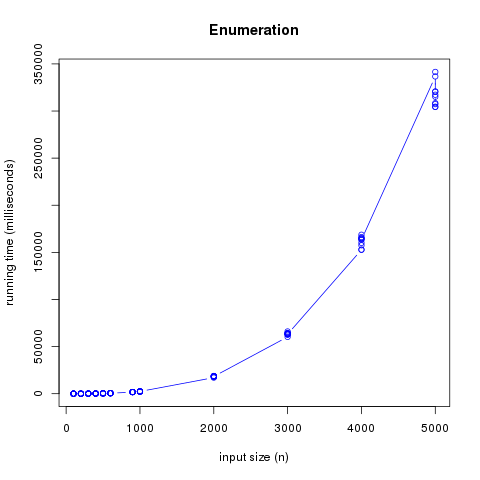
\includegraphics[width=0.50\textwidth]{runtime_enumeration.png}%
		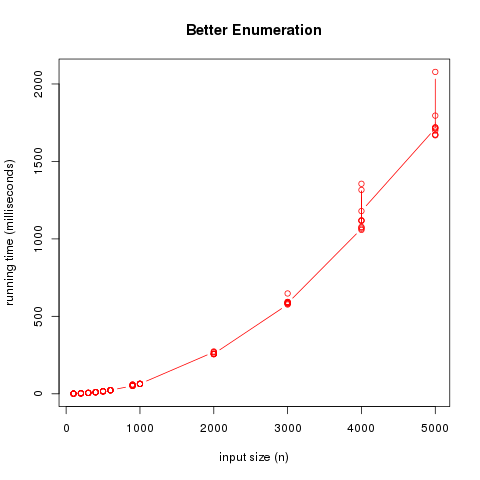
\includegraphics[width=0.50\textwidth]{runtime_better_enumeration.png}\\
		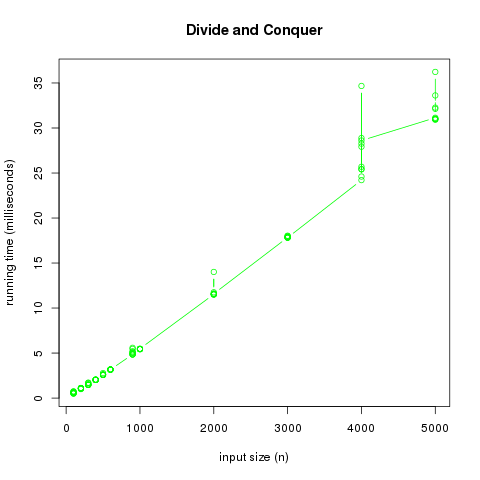
\includegraphics[width=0.50\textwidth]{runtime_divide_n_conquer.png}%
		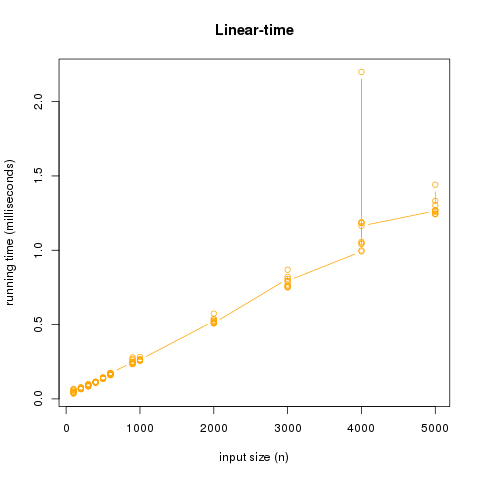
\includegraphics[width=0.50\textwidth]{runtime_linear_time.png}%
		\phantomsubcaption\label{fig:1a}%
		\phantomsubcaption\label{fig:1b}%
		\phantomsubcaption\label{fig:1c}%
		\phantomsubcaption\label{fig:1d}%	
	}%
	\label{figure1}
\end{figure}



\section{Discussion of discrepancies between experimental and theoretical running times}

\section{Largest input for each algorithm}

\section{Log-log plot}

\section{Combined algorithms running time plot}



\end{document}
